%!TEX root = ../main/main.tex

We can observe that the Strahler number is similar to a centrality measure, in a sense which, is a function who takes a node an assigns a score (with certain conditions), that's why the co-relation between Strahler number is visible. We can define the centrality measure using Strahler number in which sense, a higher Strahler number means higher centrality, it's important to remember that a potential function tell us if a centrality measure is able to root trees, in other words, if a centrality measure admits a potential function, it will roots trees if and only the potential function is simetric (not necessarily works backwards). Its valid to inquire if this centrality roots trees, we can approach this by finding a a potential function such as:
    \begin{equation}
        f_{S_{N}} (v,T) = \left\{ \begin{array}{llc}
             1 &   \text{If v is a leaf (does not have childs)}  &\\
             \\ i & \text{If all childs of v have $f_{S_{N}} (u,T) = i$} \\
             \\ i + 1 &  \text{If at least one child $u^{
             *}$ have $f_{S_{N}} (u^{*},T) = i+1$} \\
         & \text{and all the others child  have at most i} 
             \end{array}
   \right.
    \end{equation}
We can see now if this function is symmetric knowing that the concept of the Strahler number, is to represent a directed graph and measure the centrality to different contexts. We can make a counter-example for this and observe that if we consider:
\begin{center}
        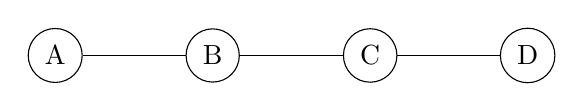
\begin{tikzpicture}
        \node[circle, draw] (A) at (0,0) {A};
        \node[circle, draw] (B) at (2,0) {B};
        \node[circle, draw] (C) at (4,0) {C};
        \node[circle, draw] (D) at (6,0) {D};

        \draw (A) -- (B) -- (C) -- (D);

    \end{tikzpicture}
\end{center}

In this example we can observe that the centrality goes to the center in the way of A to B and D to C, such that, $f(B,T_{B,A}) >  f(A,T)$ in such way that this is not symmetrical and in this sense does not root trees.

Knowing that this admits a potential function f and f is not symmetrical, by theorem it will not root trees, in other words, we can not find the root of tree in all cases with this centrality. If this centrality does not roots trees we can explore other things like if this potential function in a monoids version, such thing can't because we can observe that, this potencial function implies a monoid that is not associtative (which is not a monoid by definition), such counter-example can be drafted like:
\begin{equation}
    \max\{ x,y \}= \left\{ \begin{array}{lcc}
              \max\{x,y \} &   if  & x \neq y \\
             \\ \max\{ x,y \} + 1 & if  & x = y 
             \end{array}
   \right.
\end{equation}
This function can represent correctly the centrality of a single vertex , but, it can not represent a potential function (recursively) because is not associative, let an example be
\begin{equation}
    \max\{ 1,\max\{ 1,2 \} \} = 2\
    \max\{ \max\{ 1,1 \},2 \}  = 3\\
    \rightarrow 2 \neq 3
\end{equation}

If this centrality can not root trees this means, we can not find a root for a tree T, which can be a problem in diferent aplications.

\vspace{1cm}

\textbf{Possible Aplications}

Knowing this centrality does not root tress, in the problem of finding the root of a vector river in such way that, we can not find the \textbf{origin} of the river in all cases using this centrality.

Another apliccation is the unconditional Galton–
Watson tree which has a specific use of the Strahler number in the way that, knowing this centrality is not symetric we can  

